\documentclass[10pt]{beamer}

\usepackage{algorithm}
\usepackage[noend]{algorithmic}
\usepackage[english]{babel}
\usepackage{framed}
\usepackage[utf8]{inputenc}
\usepackage{minted}
\usepackage{xcolor}
\usepackage{xspace}

\usetheme{Copenhagen}
\setbeamertemplate{navigation symbols}{}
\setbeamertemplate{bibliography entry title}{}
\setbeamertemplate{bibliography entry location}{}
\setbeamertemplate{bibliography entry note}{}

% http://tex.stackexchange.com/a/151311/10806
\addtobeamertemplate{title page}{
  
\includegraphics[scale=0.025]{tex/img/cern}
}{}

\title{
  Machine Learning Reference Extraction\\
  Using GROBID
}
\author[Jacopo Notarstefano]{
  Jacopo Notarstefano\\
  \texttt{jacopo.notarstefano [at] cern.ch}\\
  \vspace{0.25cm}
  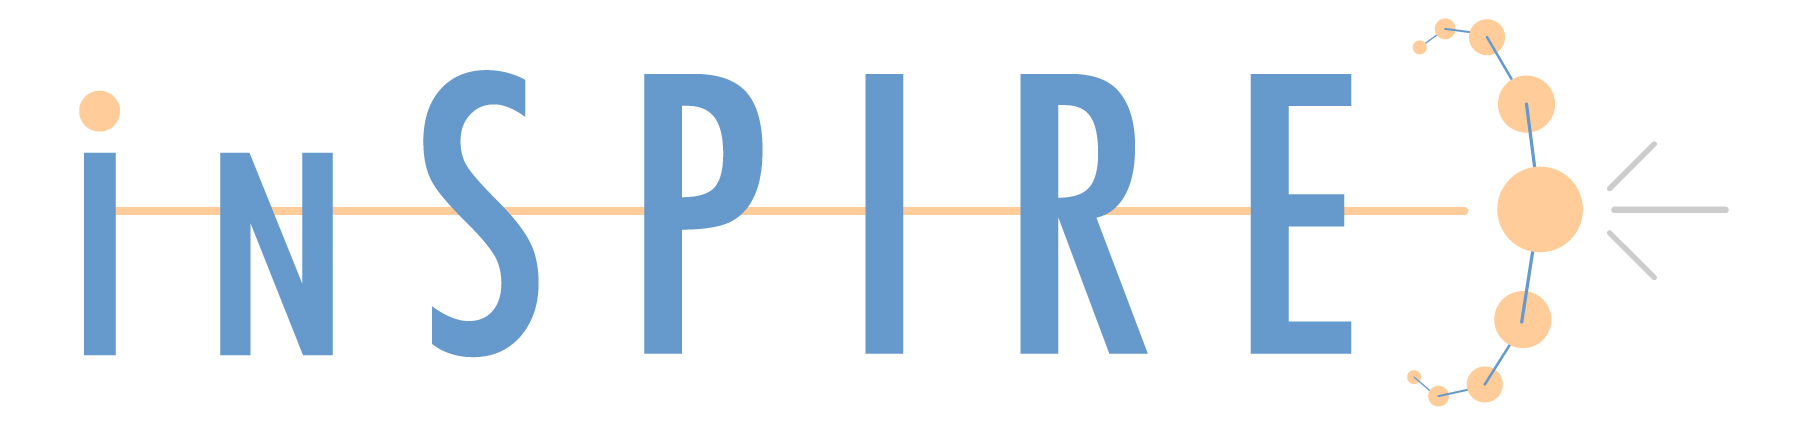
\includegraphics[scale=0.25]{tex/img/inspire}
}
\date{November 23rd, 2015}

% http://tex.stackexchange.com/a/4304/10806
\newcommand{\cpp}{C\nolinebreak\hspace{-.05em}\raisebox{.4ex}{\tiny\bf +}\nolinebreak\hspace{-.10em}\raisebox{.4ex}{\tiny\bf +}}

\definecolor{blue}{RGB}{51, 105, 232}
\definecolor{red}{RGB}{213, 15, 37}
\definecolor{yellow}{RGB}{238, 178, 17}
\definecolor{green}{RGB}{0, 153, 37}

\begin{document}
  \begin{frame}[plain]
    \titlepage
  \end{frame}

  \begin{frame}{Use cases}
    Curators often find themselves in one of the following situations:

    \vspace{0.5cm}

    \begin{enumerate}
      \item They only have the PDF of a paper, but no metadata.
      \item The source provides only part of the metadata, but they want to extract more from the PDF.
      \item They want to save the time spent entering metadata manually.
    \end{enumerate}
  \end{frame}

  \begin{frame}{Legacy: RefExtract}
    These problems were partially solved in the past by RefExtract, a series of
    heuristic based regular expressions to extract references from the output
    of \texttt{pdftotext}.

    \vspace{0.5cm}

    This solution eventually grew out of proportions and became hard to mantain, so
    we approached a library called GROBID as a better \textbf{off-the-shelf} solution.
  \end{frame}

  \begin{frame}{Future: GROBID}
    GROBID (GeneRation Of BIbliographical Data) is a machine learning library for parsing
    unstructured PDFs in structured XML documents, with a focus on technical and scientific
    publications.

    \vspace{0.5cm}

    It is a Java library that wraps Wapiti, a \cpp\xspace toolkit for segmenting and
    labeling sequences using Conditional Random Fields.

    \vspace{0.25cm}

    Its starting point is the output of \texttt{pdftoxml}, which retains much more of
    the PDF structure than \texttt{pdftotext}.

    \vspace{0.5cm}

    GROBID is widely used, for example at ResearchGate, Mendeley, HAL...
  \end{frame}

  \begin{frame}{Labeling sequences and PDFs, 1/2}
    Let's see why extracting metadata from a PDF can be reduced to labeling a sequence.
    Let's consider for example a reference:

    \vspace{0.5cm}

    \begin{framed}
      G. Isidori and F. Teubert, \textit{Status of indirect searches for New Physics with heavy flavour decays after the initial LHC run, Eur.Phys.J.Plus} \textbf{129} (2014) 40
    \end{framed}
  \end{frame}

  \begin{frame}{Labeling sequences and PDFs, 2/2}
    Extracting metadata can be seen as labeling each word with a category,
    encoded in this case as a color:

    \vspace{0.5cm}

    \begin{framed}
      \color{blue}G. Isidori and F. Teubert, \color{red}\textit{Status of indirect searches for New Physics with heavy flavour decays after the initial LHC run, \color{green}Eur.Phys.J.Plus} \color{green}\textbf{129} (2014) 40\color{black}
    \end{framed}
  \end{frame}

  \begin{frame}{GROBID architecture}
    In GROBID parlance, the \emph{knowledge} that is used to extract metadata
    from data is called a \textbf{model}. GROBID is nothing more than a
    cascade of models, each acting on the output of the previous one.

    \vspace{0.5cm}

    \makebox[\textwidth][c]{
      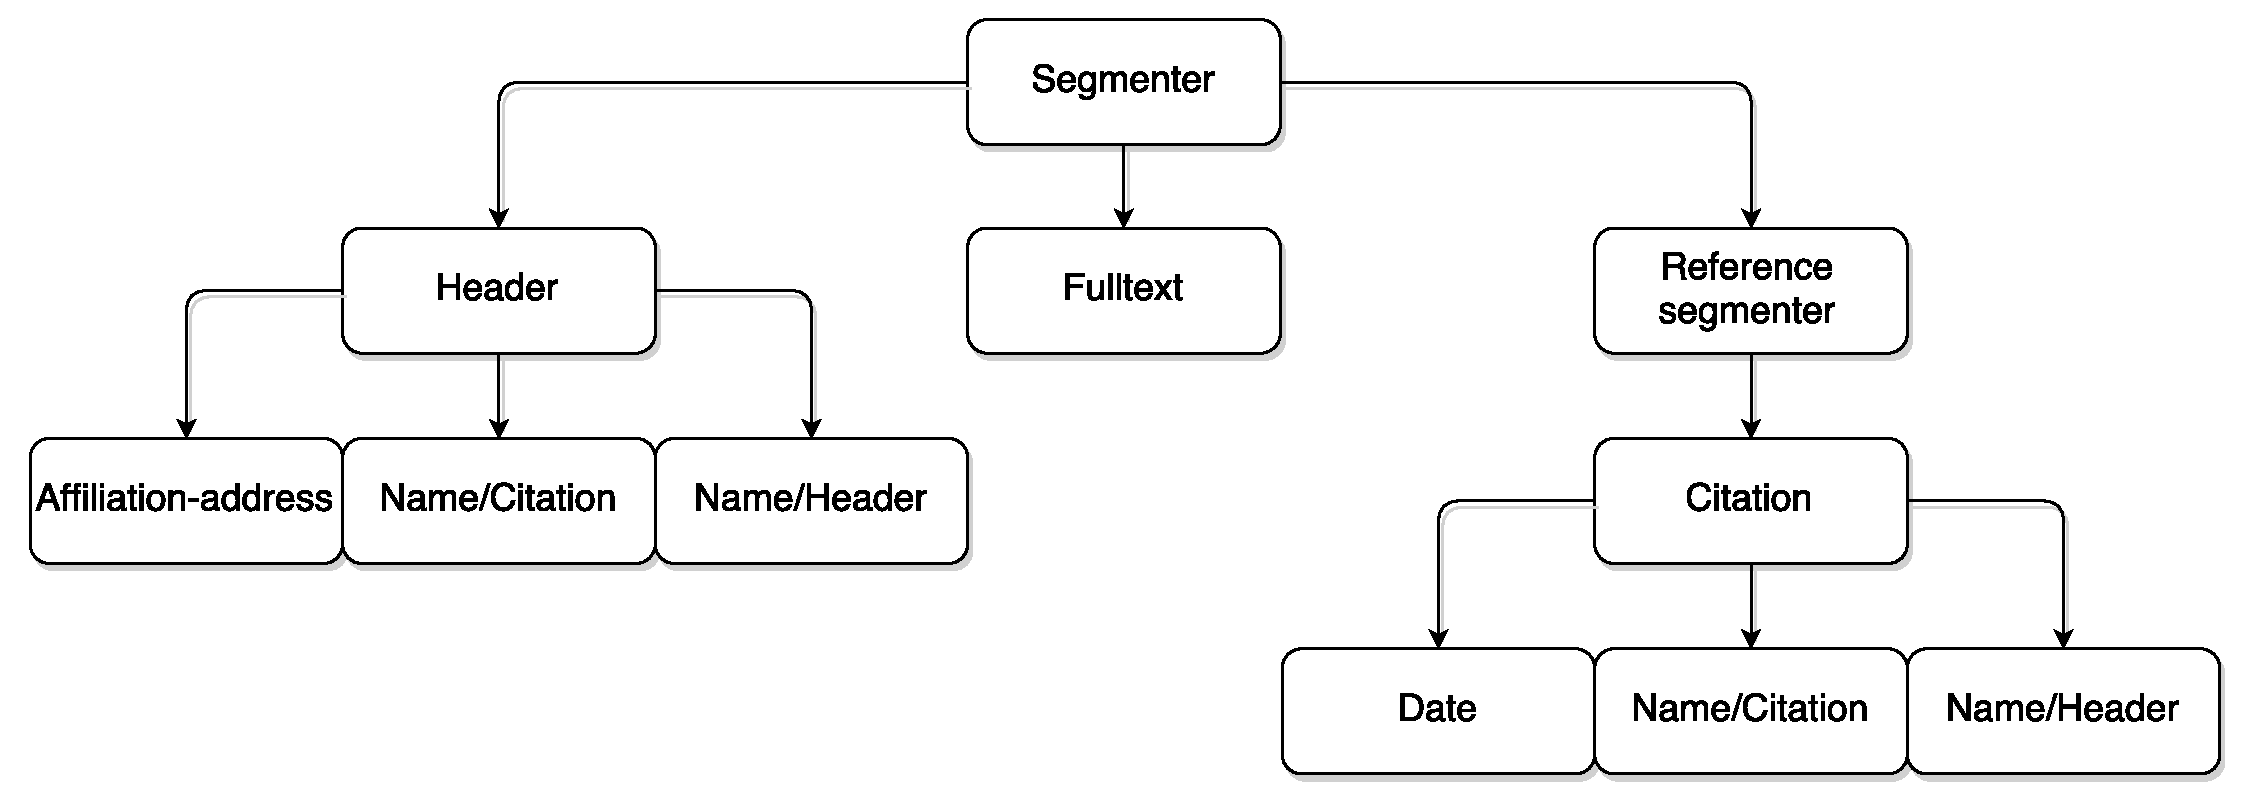
\includegraphics[width=0.9\textwidth]{tex/img/cascade.pdf}
    }
  \end{frame}

  \begin{frame}{GROBID's output: TEI}
    TEI (Text Encoding Initiative) publishes a set of guidelines which specify
    encoding methods for machine-readable texts. By extension, we will call
    ``TEI'' the format described by these guidelines. GROBID's output conforms
    to a subset of TEI.

    \vspace{0.5cm}

    \inputminted[fontsize=\tiny]{xml}{tex/src/reference.xml}
  \end{frame}

  \begin{frame}{GROBID credits}
    GROBID is the work of Patrice Lopez, developer at INRIA. It has been adapted
    to papers from the HEP community by Joseph Boyd as part of his Master's Thesis
    for EPFL, under the supervision of Gilles Louppe, Senior Fellow at Inspire.

    \vspace{0.5cm}

    In particular, Joseph added to GROBID the concept of a \emph{collaboration},
    such as ATLAS or CMS, and improved considerably the accuracy of GROBID's
    models by providing lots of training data, taken from Inspire.
  \end{frame}

  \begin{frame}{Caveat emptor}
    \begin{framed}
      ``Converting PDF to XML is a bit like\\ converting hamburgers into cows.''

      \vspace{0.25cm}

      \hspace*\fill{--- Michael Kay}
    \end{framed}

    \vspace{0.5cm}

    That is, GROBID is not magic: it will misclassify things in various ways,
    and requires lots of training data to function properly.
  \end{frame}

  \begin{frame}[plain]
    \makebox[\textwidth][c]{
      \Huge DEMO
    }
  \end{frame}
\end{document}
